\section{EnDASH - A Mobility Adapted Energy Efficient ABR Video Streaming for Cellular Networks}
From the observations in previous sections, we design an ABR algorithm, EnDASH, which aims to reduce the radio's energy consumption during the video streaming. EnDASH reads the environment using different parameters and try to predict the future. Based on the prediction, it schedules segment downloading in a way so that it reduces the overall energy consumption. EnDASH does not directly schedule the video segments; instead, it changes the available buffer (which is a parameter) in the player, and the DASH controller schedules the segment downloading according to the buffer length.
\subsection{EnDASH System}
EnDASH first predicts the expected throughput for the short future ($t$) from the past and based on predicted throughput, and it decides the buffer length for $t$ duration. Later on, it also decides the bitrate based on the past information and current buffer length, and predicted throughput. EnDASH use three machine learning engine for each step.

\begin{figure}[!h]
	\centering
	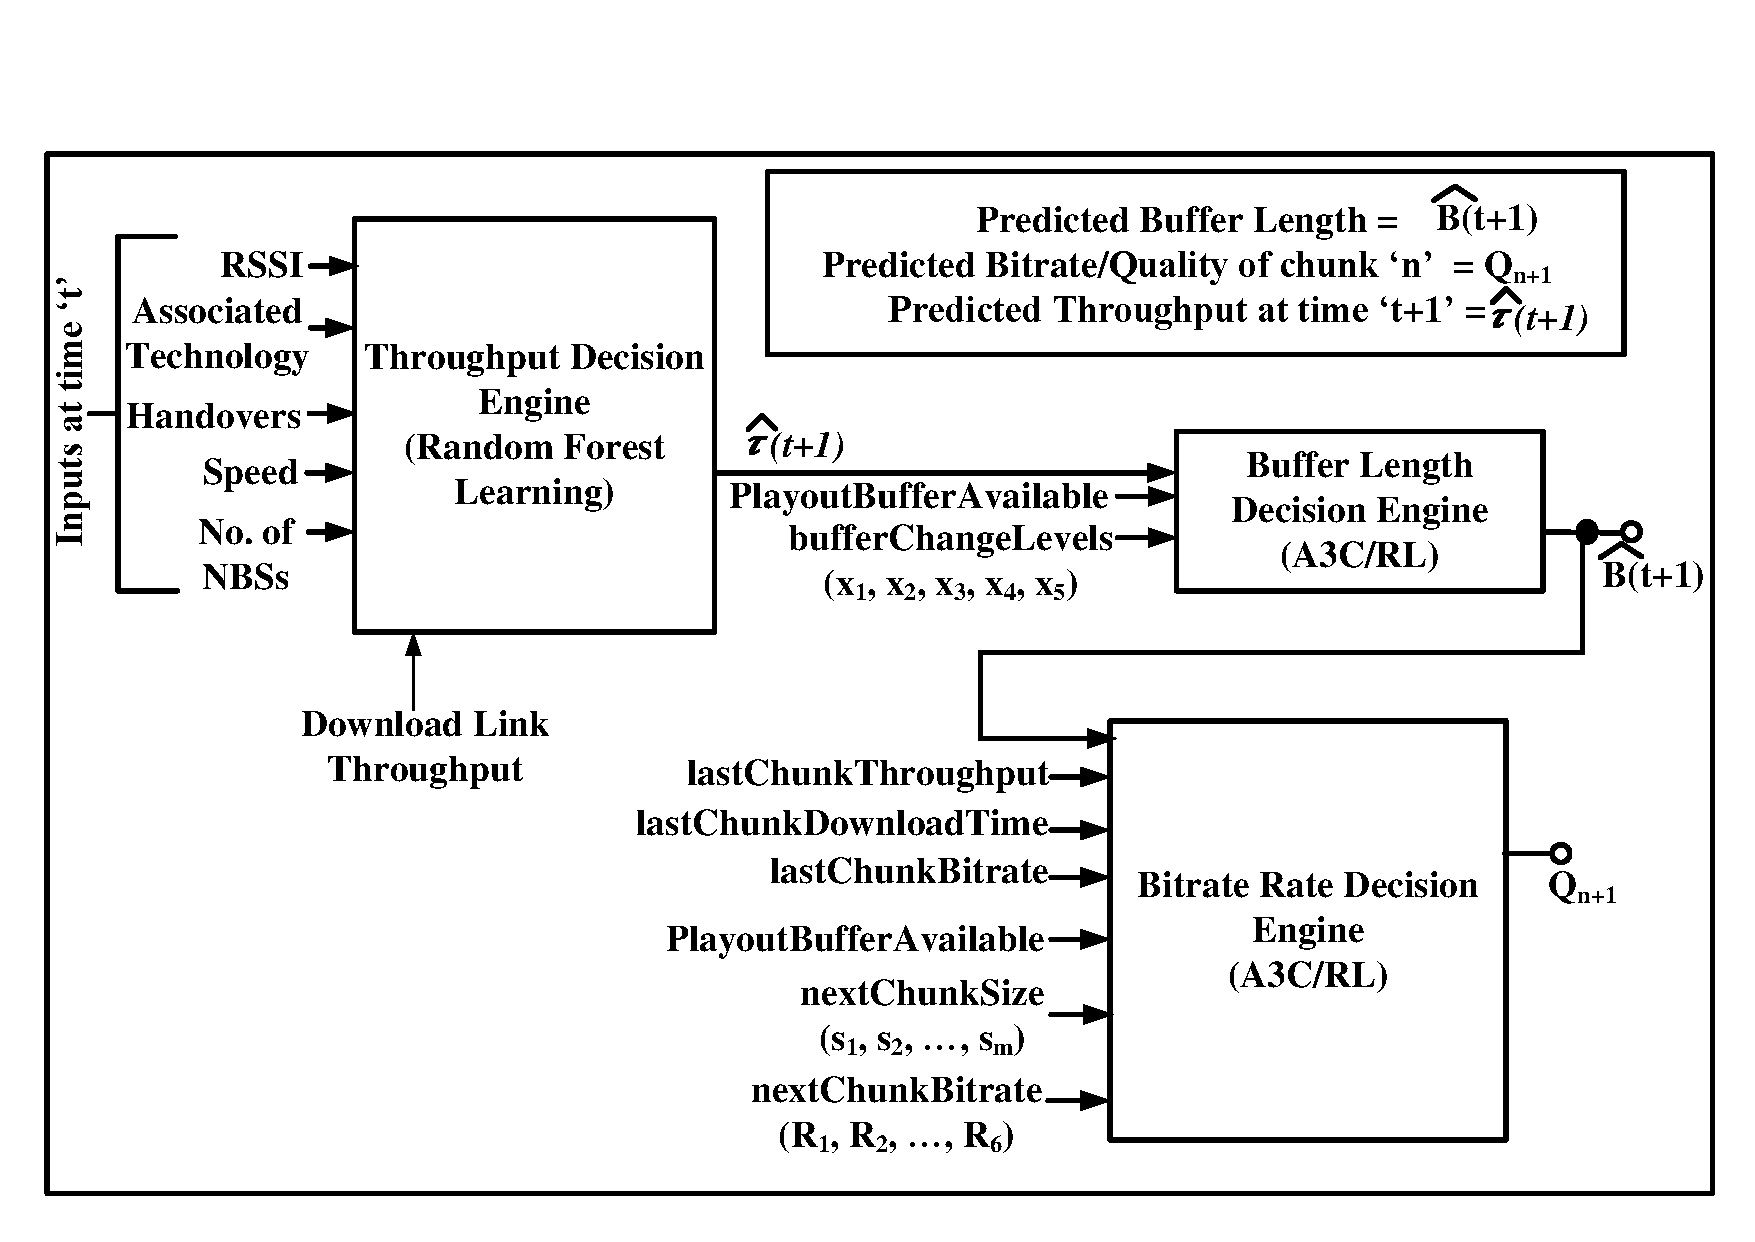
\includegraphics[width=0.7\linewidth]{img/EnDASH/EnDASH_system}
	\caption{Composite Representation of the EnDASH model; a cascaded model where the predicted throughput acts as an input network state to the Actor Critic RL based decision
		engine}
	\label{fig:endash:system}
\end{figure}

\subsubsection{The throughput prediction engine}
EnDASH uses random forest learning to predict the expected throughput for the next 30sec from past information. It uses features like the device's speed, cellular RSSI, current technology, handovers. As the features sets are enormous, we feed only the $\mathrm{25^{th}}$, $\mathrm{75^{th}}$, and $\mathrm{90^{th}}$ percentile points, median and mean from its historical data of each feature.
\subsubsection{The Buffer Length Decision Engine}
The buffer length decision engine uses an A3C RL-based deep neural network to determine the optimal buffer length. It takes the predicted throughput, last buffer length, and possible steps to change buffer length. It returns the decision whether buffer length needs to increase or decrease or keep the same. We use a linear weighted function of energy savings during the training phase concerning a baseline ABR algorithm and the QoE score as the reward.

The throughput prediction engine and the buffer length prediction engine run only once every $t$ time and in this order only.

\subsubsection{The Bitrate Decision Engine}
EnDASH uses another A3C RL based deep neural network to estimate the quality of the next chunk based on several playbacks related parameters and the buffer length, similar to the parameters used in Pensieve~\cite{mao2017neural}. It runs before fetching the next segment and uses QoE as the reward during the training phase.

The complete architecture of the EnDASH decision engine is presented in Fig.~\ref{fig:endash:system}.

\begin{figure}[!h]
	\begin{minipage}[t]{0.48\linewidth}
		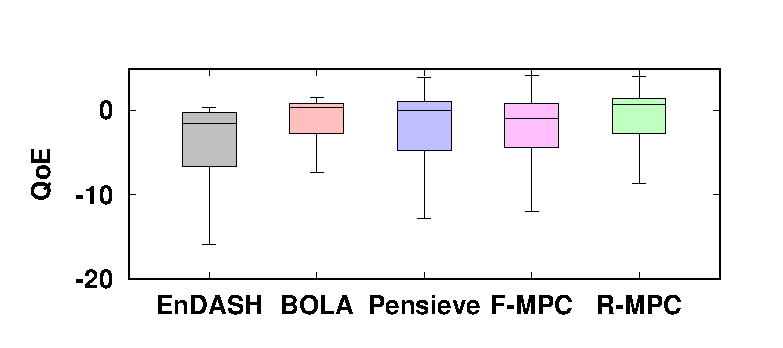
\includegraphics[width=\linewidth]{img/EnDASH/QoE}
		\caption{\label{fig:endash:qoe}}
	\end{minipage}\hfill
	\begin{minipage}[t]{0.48\linewidth}
		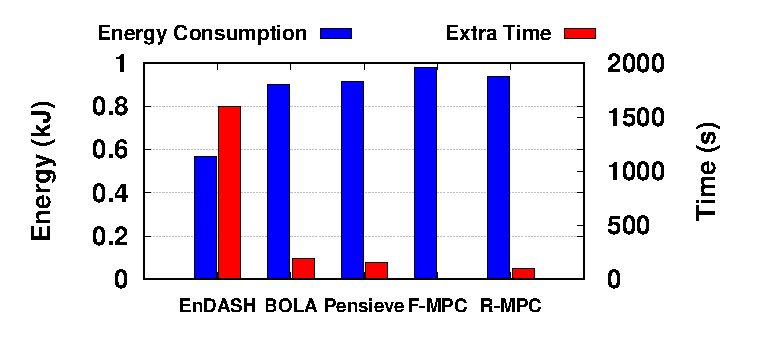
\includegraphics[width=\linewidth]{img/EnDASH/EnergyConsumption}
		\caption{\label{fig:endash:energy}}
	\end{minipage}
\end{figure}
\subsection{Evaluation}
We train and test all these three engines in an emulation platform with the data we collected from various commodity smartphones like Moto G5, Micromax canvas over Airtel, Reliance Jio, and Vodaphone. Once training and testing are completed for each individual module, we run experiments in our emulation based testbed, comparing QoE performance and energy saving of EnDASH. In Fig.~\ref{fig:endash:qoe} we compare the performance in terms of QoE with modern ABR algorithms. EnDASH slightly compromises the QoE; however, it saves a lot of energy. In Fig.~\ref{fig:endash:energy}, we plot the energy uses and possible run time with respect to Fast-MPC, and it turns out that video can be played for another 20-25 minutes with EnDASH compared to Fast-MPC.
